% !TEX root = ../paper.tex

%\section{Background}
%In this section, we describe MCR process based on Gerrit system. Then, we describe the background behind our approach composed of text mining techniques using VSM and euclidian distance and prediction evaluation techniques. 
\dan{this section seems to only cover MCR. We could have this be a Background section with this and the other subsequent sections moved to sub-sections}
\section{Modern Code Review Process}

An overview of MCR process based on Gerrit system is shown in Fig. \ref{fig:process}. The grey area shows the review process of the system which composed of four main steps. (1) an author creating a patch and submitting a set of new or modified files as a review request to Gerrit system. (2) reviewers examine the proposed code changes for defects or concerns. (3) reviewers provide comments to the author. The author creates a revised proposed change according to the comments then re-submits for review. Then, reviewers will examine the revised proposed change. If the revision is not approved, reviewers provide comments to fix and the process continues until reviewers can determine that a proposed change can be merged into the project (approved change) or should not be merged (reject the change). 

According to this process, reviewers' comments are the most important factor in determining software quality. In particular, McIntosh et. al. \cite{Mcintosh} found that components which were reviewed without discussion are likely to contain bugs. However, tools supporting MCR allow reviewers to freely write messages to the author (and other reviewers) and frequently comments are superficial or do not clearly identify defects or relevant issues (e.g. design suggestions, coding styles, etc.) for the proposed change and are thus of questionable usefulness. For example a comment may relate to something outside the scope of the proposed change, perhaps personal issues or inter-personal communication (e.g. "Keep up the good work!"). Microsoft developers reported that they only focus on minor logic errors rather than discussing deeper design\cite{Bacchelli2013a} issues. Our observations of the Qt project also correspond to this finding. We found some comments are superficial and unhelpful to the proposed changes. For example, the superficial and unconfident comment shown in Fig. \ref{fig:example}(a) is indeed within the scope of the proposed change yet provides little useful information. While the comment in Fig. \ref{fig:example}(b) about using the version control system (in this case Git) is clearly out of scope and not directly useful for the proposed change. 

\begin{figure}[!t]
\centering
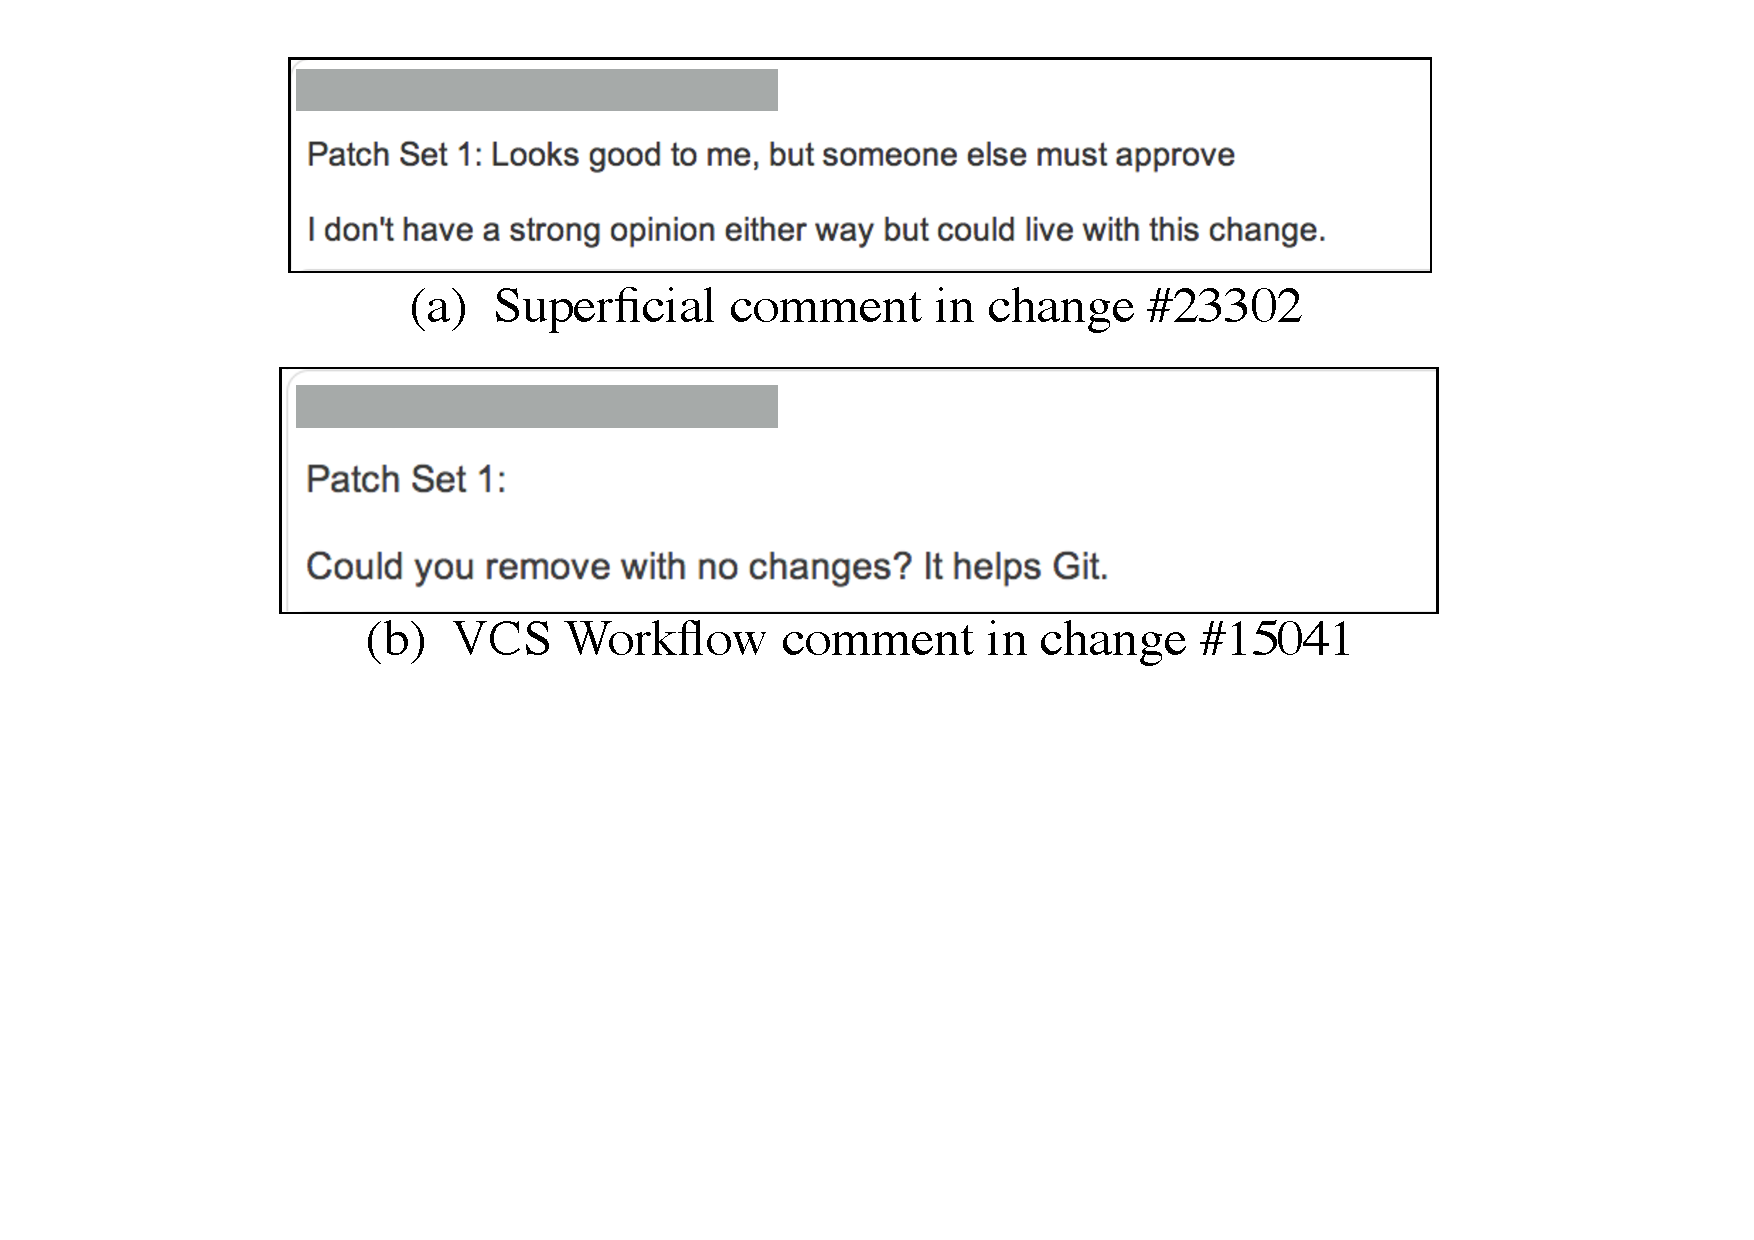
\includegraphics[scale=0.4, trim= 100 250 0 0, clip=true]{comment_examples}
\caption{Examples of comment in code reviews of Qt project.}
\label{fig:example}
\end{figure}

